% ================================================================
%  Professional Academic Symposium Poster  (A0 portrait, single page)
%  — Flowing layout with tcolorbox, Palatino serif
% ================================================================
\documentclass[a0paper]{article}

\usepackage[left=2.2cm, right=2.2cm, top=0pt, bottom=1.5cm]{geometry}
\usepackage[utf8]{inputenc}
\usepackage[T1]{fontenc}
\usepackage{mathpazo}
\usepackage[scaled=0.88]{helvet}
\usepackage{courier}
\usepackage{amsmath,amssymb}
\usepackage{graphicx}
\usepackage{tikz}
\usepackage{enumitem}
\usepackage{xcolor}
\usepackage{microtype}
\usepackage{multicol}
\usepackage{tcolorbox}

\tcbuselibrary{skins}
\usetikzlibrary{calc}

\pagestyle{empty}
\graphicspath{ {../tex/images/} }

% ---------------------------------------------------------------
%  Colour palette
% ---------------------------------------------------------------
\definecolor{DeepNavy}{HTML}{0B1D3A}
\definecolor{SlateBlue}{HTML}{1E3A5F}
\definecolor{SteelBlue}{HTML}{3C6E9F}
\definecolor{PaleIvory}{HTML}{FAFAF6}
\definecolor{WarmGray}{HTML}{F2F0EC}
\definecolor{DarkCharcoal}{HTML}{2A2A2A}
\definecolor{MutedGold}{HTML}{B8922F}
\definecolor{ForestGreen}{HTML}{1D7A47}
\definecolor{RuleGray}{HTML}{D3D0CA}
\definecolor{LightSteel}{HTML}{EBF0F7}

% ---------------------------------------------------------------
%  Font sizes for A0
% ---------------------------------------------------------------
\renewcommand{\normalsize}{\fontsize{22}{29}\selectfont}
\newcommand{\smallbody}{\fontsize{19}{25}\selectfont}
\newcommand{\tinybody}{\fontsize{18}{24}\selectfont}

% ---------------------------------------------------------------
%  tcolorbox styles
% ---------------------------------------------------------------
\newtcolorbox{posterbox}[1]{%
  enhanced,
  colback=PaleIvory,
  colframe=RuleGray,
  boxrule=0.8pt,
  arc=6pt,
  left=20pt, right=20pt, top=14pt, bottom=14pt,
  fonttitle=\sffamily\bfseries\fontsize{32}{38}\selectfont\color{white},
  coltitle=white,
  colbacktitle=SlateBlue,
  attach boxed title to top left={yshift=-2pt, xshift=0pt},
  boxed title style={
    enhanced, arc=5pt, outer arc=5pt,
    boxrule=0pt, left=12pt, right=12pt, top=5pt, bottom=5pt,
  },
  title={#1},
  before skip=6pt,
  after skip=6pt,
}

\newtcolorbox{hlbox}{%
  enhanced,
  colback=LightSteel,
  colframe=SteelBlue!60,
  boxrule=1pt,
  arc=5pt,
  left=14pt, right=14pt, top=12pt, bottom=12pt,
}

\newtcolorbox{resultbox}{%
  enhanced,
  colback=ForestGreen!4,
  colframe=ForestGreen!50,
  boxrule=1.2pt,
  arc=5pt,
  left=14pt, right=14pt, top=12pt, bottom=12pt,
}

\newtcolorbox{eqbox}{%
  enhanced,
  colback=SteelBlue!4,
  colframe=SteelBlue!35,
  boxrule=0.8pt,
  arc=4pt,
  left=12pt, right=12pt, top=10pt, bottom=10pt,
}

\newtcolorbox{conclusionbox}{%
  enhanced,
  colback=DeepNavy,
  colframe=MutedGold,
  boxrule=1.5pt,
  arc=6pt,
  left=22pt, right=22pt, top=18pt, bottom=18pt,
}

\newcommand{\step}[1]{%
  \tikz[baseline=(S.base)]{%
    \node[circle, fill=SlateBlue, text=white,
          font=\sffamily\bfseries\fontsize{22}{26}\selectfont,
          minimum size=32pt, inner sep=0pt] (S) {#1};%
  }\;%
}

% ---------------------------------------------------------------
\begin{document}
\normalsize\color{DarkCharcoal}

% ===============================================================
%  HEADER BANNER  (navy band tall enough for all fields)
% ===============================================================
\noindent
\begin{tikzpicture}[remember picture, overlay]
  \fill[WarmGray]
    (current page.north west) rectangle (current page.south east);
  \fill[DeepNavy]
    (current page.north west) rectangle
    ([yshift=-19.5cm]current page.north east);
  \fill[MutedGold]
    ([yshift=-19.2cm]current page.north west) rectangle
    ([yshift=-19.5cm]current page.north east);
\end{tikzpicture}%
%
\vspace*{1.5cm}
\begin{center}
  {\bfseries\fontsize{60}{70}\selectfont\color{white}%
   Block-Sparse Attention with Prefix Caching:\\[0.25em]
   Integrating MInference into vLLM via the\\[0.25em]
   PagedAttention--Sparsity Isomorphism\par}

  \vspace{1.0cm}
  {\itshape\fontsize{34}{40}\selectfont\color{MutedGold}%
   University of Macau\par}

  \vspace{0.9cm}
  {\fontsize{32}{40}\selectfont\color{white}%
   \renewcommand{\arraystretch}{1.9}%
   \begin{tabular}{@{}r@{\;\;}l@{\hspace{4cm}}r@{\;\;}l@{}}
     \textsf{\textbf{Student: PO HIU LAM (DC227620)}} & 
    %  & \textsf{\textbf{Student No.: DC227620}} &  \\
      \textsf{\textbf{Advisor: Huanle Xu}} &
    %  & \textsf{\textbf{Co-Advisor:}} & \rule{5.5cm}{0.4pt} \\
   \end{tabular}\par}
\end{center}

\vspace{5.5cm}

% ===============================================================
%  TWO-COLUMN CONTENT
% ===============================================================
\setlength{\columnsep}{1.6cm}
\begin{multicols}{2}

% ---------------------------------------------------------------
%  I.  PURPOSE
% ---------------------------------------------------------------
\begin{posterbox}{I.\;\;Purpose of the Project}
  Large Language Models increasingly demand long-context reasoning
  (128K--10M tokens). In production, \textbf{shared system prompts}
  are identical across requests, yet must be reprocessed every time
  ---a fundamental bottleneck.

  \vspace{0.3em}
  Two complementary optimisations exist independently:
  \begin{itemize}[leftmargin=1.6em, itemsep=0.25em, topsep=0.2em]
    \item \textbf{PagedAttention} (vLLM)\,: Stores KV caches in
      fixed-size blocks; \textit{prefix caching} computes shared KV
      once and reuses it across requests.
    \item \textbf{MInference}\,: Exploits the sparsity of attention
      weights ($<$5\%\ non-zero), reducing FLOPs by up to
      \textbf{95\%} via dynamic block-sparse attention.
  \end{itemize}

  \vspace{0.3em}
  \begin{hlbox}
    \textcolor{SlateBlue}{\textbf{Problem.}}\;
    These systems are \textit{fundamentally incompatible}.
    MInference requires equal-length $Q, K, V$ processed from
    scratch---no mechanism to accept a pre-computed KV cache.

    \vspace{0.25em}
    \textcolor{SlateBlue}{\textbf{Objective.}}\;
    Identify the structural isomorphism between block-sparse
    attention and PagedAttention, enabling sparse attention +
    prefix caching for the first time.
  \end{hlbox}
\end{posterbox}

% ---------------------------------------------------------------
%  II.  KEY INSIGHT
% ---------------------------------------------------------------
\begin{posterbox}{II.\;\;The PagedAttention--Sparsity Isomorphism}
  Block-sparse attention is \textbf{naturally compatible} with
  PagedAttention's paged memory layout:
  \begin{itemize}[leftmargin=1.6em, itemsep=0.2em, topsep=0.2em]
    \item Block-sparse attention partitions the attention matrix
      into blocks of size $b\!\times\!b$; column $c$ spans KV tokens
      $[cb,\,(c\!+\!1)b)$.
    \item PagedAttention stores KV vectors in physical pages of $B$
      tokens; page $\phi(c)$ stores tokens $[cB,\,(c\!+\!1)B)$.
  \end{itemize}

  \vspace{0.2em}
  Setting $b = B$, the correspondence is exact:
  \begin{eqbox}
    \centering
    \fontsize{30}{36}\selectfont
    $\text{Attention Block}\ (r,\,c)
    \;\longleftrightarrow\;
    \text{Physical KV Page}\ \phi(c)$
  \end{eqbox}

  \vspace{0.3em}
  \textbf{No data reorganisation, no gather operation, no
  auxiliary structures.} The block table $\phi$ provides $O(1)$
  access to the exact physical memory for any block.
  Selective page access reduces I/O dramatically:
  \[
    \mathcal{P}_{\text{load}}
    = \bigl\{\phi(c) : \exists\, r\;\text{s.t.}\;(r,c)
      \in \hat{\mathcal{I}}\bigr\}
    \quad
    |\mathcal{P}_{\text{load}}| \leq k_b \!\cdot\! \tfrac{n_q}{B}
    \;\ll\; \tfrac{n_p\!+\!n_q}{B}\!\cdot\!\tfrac{n_q}{B}
  \]

  \vspace{0.2em}
  \begin{center}
    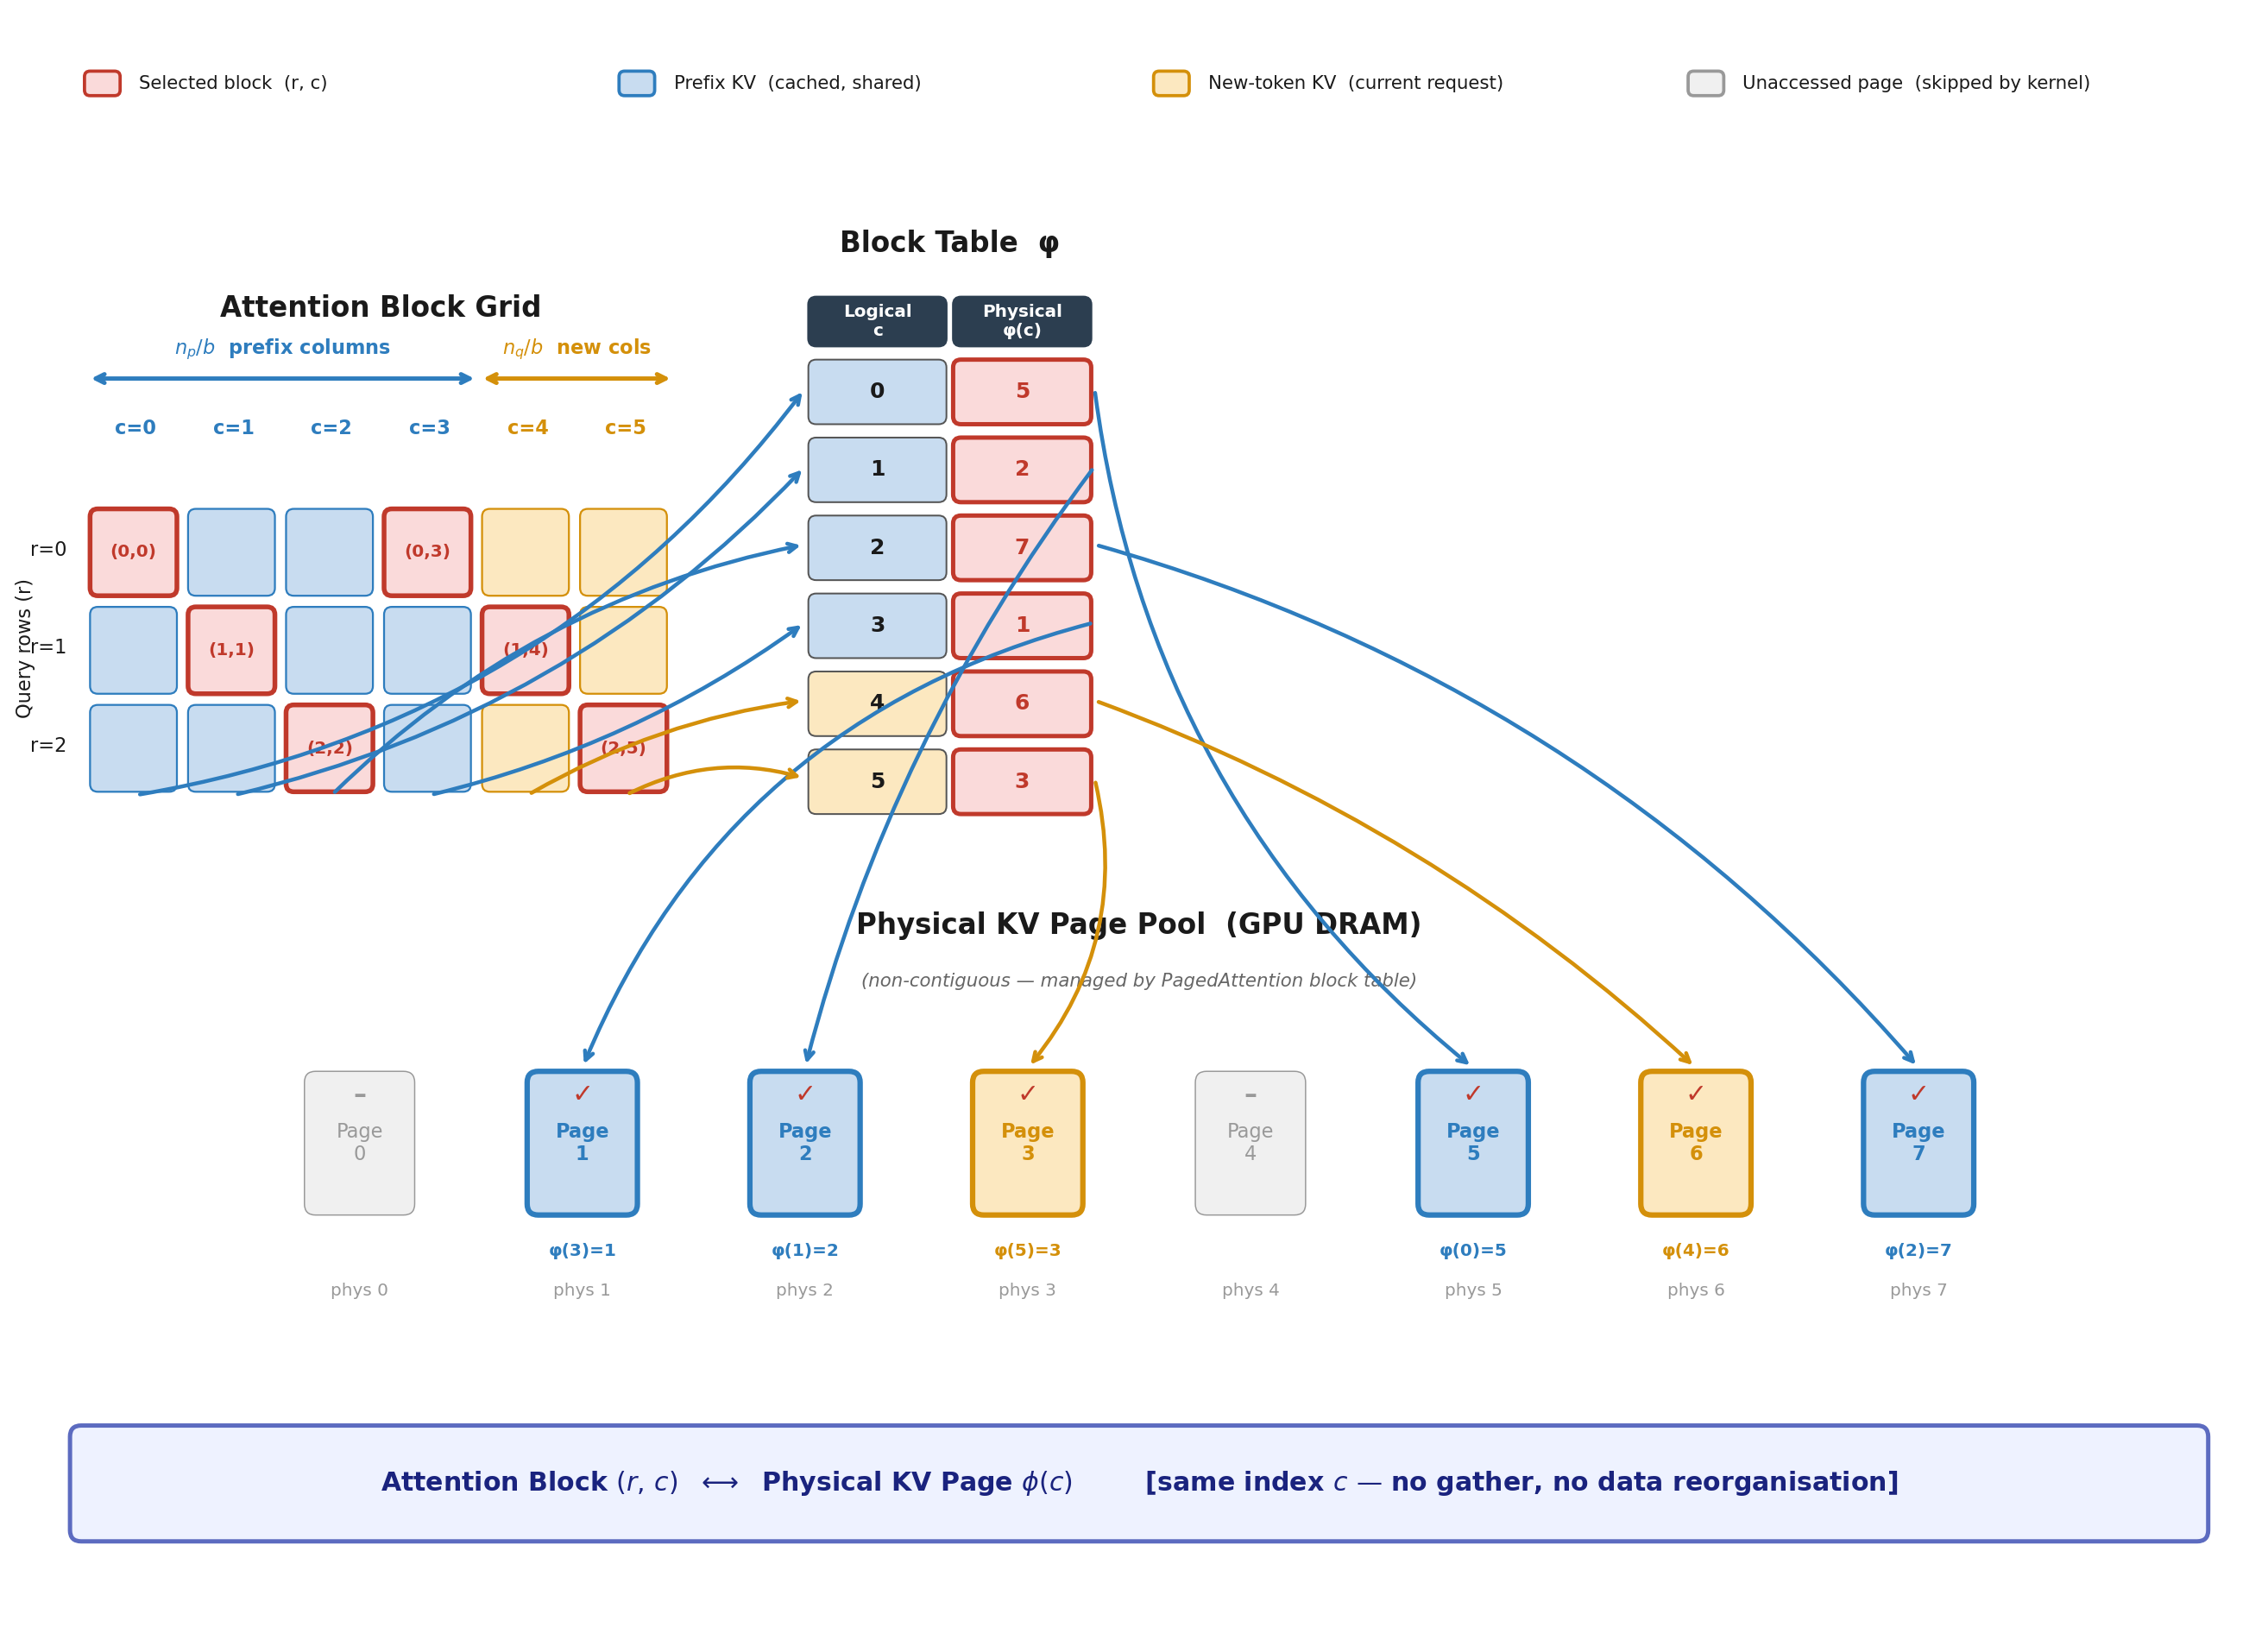
\includegraphics[width=0.85\linewidth]{isomorphism.png}
  \end{center}
  \vspace{-0.2em}
  {\smallbody\itshape\centering
   Figure 1.\; KV vectors for block $(r,c)$ are precisely stored
   in physical page $\phi(c)$.\par}

  \vspace{0.4em}
  \textbf{Prefix caching and shared pages.}\;
  Shared prefix pages are stored once in physical memory and
  referenced by multiple requests via the block table. Each
  request's importance predictor independently selects a different
  subset of prefix pages depending on its query content.
  Pages not selected are simply not accessed---with zero overhead.

  \vspace{0.4em}
  \begin{hlbox}
    \textcolor{SlateBlue}{\textbf{Contributions}}
    \begin{enumerate}[leftmargin=1.6em, itemsep=0.15em, topsep=0.15em]
      \item Identify the fundamental incompatibility between
        MInference and KV cache systems.
      \item Formalise the structural isomorphism between
        block-sparse column indices and PagedAttention page addresses.
      \item Integrate MInference's predictor into vLLM, enabling
        sparse attention over prefix-cached KV pages for the
        first time.
      \item Demonstrate 63\% latency reduction with near-identical
        output fidelity.
    \end{enumerate}
  \end{hlbox}
\end{posterbox}

% Column break
\vfill\null
\columnbreak

% ---------------------------------------------------------------
%  III.  METHODOLOGY
% ---------------------------------------------------------------
\begin{posterbox}{III.\;\;Methodology}
  The system integrates into vLLM with three components:

  \vspace{0.4em}
  \step{1}\textbf{Online Importance Predictor}

  \vspace{0.15em}
  Coarse block importance via mean-pooled $Q$ and $K$ over the
  full rectangular grid:
  \[
    \bar{Q}_r = \frac{1}{b}\!\sum_{i=rb}^{(r+1)b}\! Q_i,\;\;
    \bar{K}_c = \frac{1}{b}\!\sum_{j=cb}^{(c+1)b}\! K_j,\;\;
    \hat{A}_{rc} = \frac{\bar{Q}_r \bar{K}_c^\top}{\!\sqrt{d_h}}
  \]
  Top-$k_b$ columns per query row yield $\hat{\mathcal{I}}$.

  \vspace{0.5em}
  \step{2}\textbf{Sparse Page Selector}

  \vspace{0.15em}
  Translates $\hat{\mathcal{I}}$ into physical pages via direct
  block-table lookup:
  \[
    \mathcal{C} = \{c : \exists\, r\;\text{s.t.}\;(r,c)
      \in \hat{\mathcal{I}}\}
    \;\xrightarrow{\;\phi\;}
    \;\{\phi(c) : c \in \mathcal{C}\}
  \]
  At 5\% sparsity $\Rightarrow$ \textbf{20$\times$ reduction}
  in pages accessed.

  \vspace{0.5em}
  \step{3}\textbf{Block-Sparse FlashAttention Kernel}

  \vspace{0.15em}
  Online softmax over selected blocks only; unselected blocks
  incur \textbf{zero computation}:
  \[
    O_r \approx
    \frac{\sum_{c \in \hat{\mathcal{I}}_r}
          e^{S_{rc} - m_r}\,V_c}
         {\sum_{c \in \hat{\mathcal{I}}_r}
          e^{S_{rc} - m_r}}
  \]
\end{posterbox}

% ---------------------------------------------------------------
%  IV.  FINDINGS
% ---------------------------------------------------------------
\begin{posterbox}{IV.\;\;Findings}
  \textbf{Theoretical Speedup.}

  \vspace{0.15em}
  \begin{eqbox}
    \centering
    $\dfrac{t_{\text{proposed}}}{t_{\text{MInference}}}
    \;=\; \dfrac{n_q}{n_p + n_q}$
    \qquad As prefix grows, latency $\to 0$.
  \end{eqbox}

  \vspace{0.35em}
  \textbf{Empirical Results}\; (NVIDIA RTX~3090, \texttt{bf16}):

  \vspace{0.25em}
  \begin{center}
    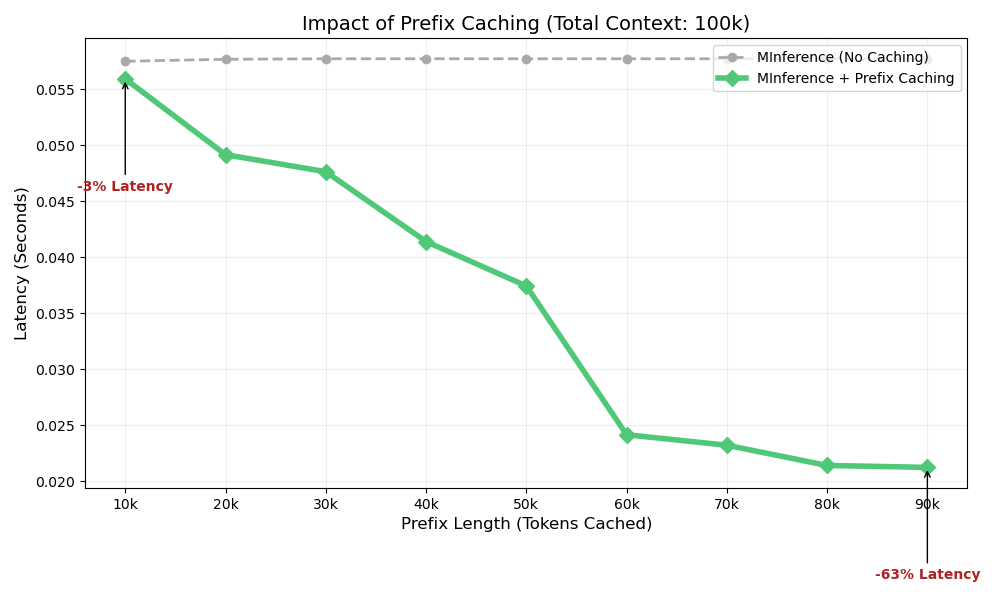
\includegraphics[width=0.88\linewidth]{Figure_2.png}
  \end{center}
  \vspace{-0.3em}
  {\smallbody\itshape\centering
   Figure 2.\; Latency at 100K context.\par}

  \vspace{0.25em}
  \begin{center}
    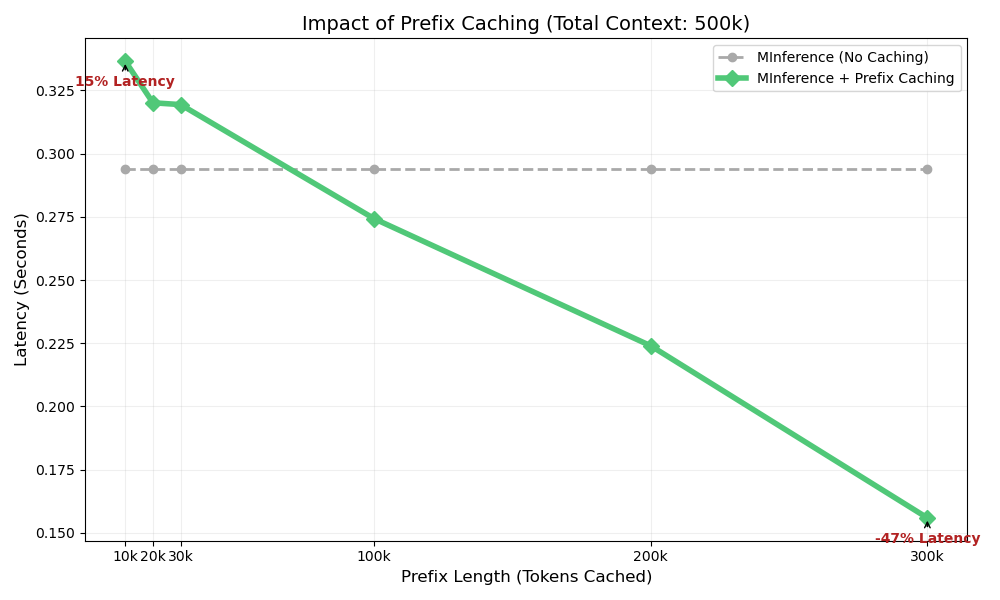
\includegraphics[width=0.88\linewidth]{Figure_3.png}
  \end{center}
  \vspace{-0.3em}
  {\smallbody\itshape\centering
   Figure 3.\; Latency at 500K context.\par}

  \vspace{0.35em}
  \begin{resultbox}
    \textbf{Key Results}
    \begin{itemize}[leftmargin=1.6em, itemsep=0.2em, topsep=0.15em]
      \item \textbf{63\% reduction} in attention kernel latency
        (100K tokens, 90K prefix cache).
      \item Near-identical output fidelity:
        $\max|\Delta| \approx 2\!\times\!10^{-3}$ (\texttt{bf16}).
      \item Speedup scales \textbf{monotonically} with prefix length.
      \item Figures are a \textit{lower bound}---end-to-end speedup
        is larger (MLP savings excluded).
    \end{itemize}
  \end{resultbox}
\end{posterbox}

\end{multicols}

\vspace{0.15cm}

% ===============================================================
%  CONCLUSION + REFERENCES  (expanded footer)
% ===============================================================
\begin{conclusionbox}
  {\sffamily\bfseries\fontsize{34}{40}\selectfont\color{white}%
   Conclusion\par}
  \vspace{0.5em}
  {\color{white!93}\normalsize
  This work identifies and formalises the
  \textbf{PagedAttention--block-sparsity isomorphism}: the column
  index of an attention block corresponds directly to the physical
  KV page $\phi(c)$ in PagedAttention's block table. This natural
  alignment enables block-sparse attention to operate directly over
  paged, prefix-cached KV memory---without data reorganisation or
  auxiliary structures. By integrating MInference's importance
  predictor into vLLM, the system selectively attends only to the
  most important pages per query row, achieving up to
  \textbf{63\% latency reduction} while maintaining near-identical
  output fidelity. This isomorphism constitutes a general
  \textbf{design principle}: any block-structured KV memory
  management system can directly leverage block-level importance
  scores to guide selective attention computation.\par}

  \vspace{0.6em}
  {\sffamily\bfseries\fontsize{28}{34}\selectfont\color{MutedGold}%
   Limitations \& Future Work\par}
  \vspace{0.35em}
  {\color{white!85}\normalsize
  The primary limitation is the overhead of online importance
  prediction, which grows as $O((n/b)^2 d_h)$ and may become
  non-trivial for extremely long contexts ($n > 1\text{M}$).
  Future work includes hierarchical prediction schemes, learned
  static masks per head, and formal end-to-end evaluation on
  long-context benchmarks (RULER, InfiniteBench).\par}
\end{conclusionbox}

\end{document}
